\chapter{یک راهنما}\label{chp:chap4}
\thispagestyle{empty}
\rhead{\leftmark}
\section{نمونه لغات}
\begin{thm}\label{thm:a}
اگر $A$ و $B$ آن‌گاه $C$.
\end{thm}
در قضیه~\ref{thm:a} داریم ... \\
کلمه

برای وارد کردن یک واژه از دستور 
\lr{glspl}
باید استفاده نمود. مثل واژه 
\glspl{RandomVariable}
که اگر در فایل \lr{\TeX}  آن نگاه کنید، مشاهده می‌کنید که برای وارد کردن واژه  \glspl{RandomVariable} از دستور \lr{glspl} استفاده شده است. در ضمن  در اولین استفاده از این واژه، معادل انگلیسی آن نیز پاورقی خورده است.  و اکنون واژه \glspl{Optimization}  را تعریف می‌کنیم. 

از اختصارات، اختصارات \gls*{BAN} و \gls{CDMA} را وارد می‌کنیم. برای بار اول پاورقی می‌خورد. اما برای بار دوم پاورقی زده نمی‌شود. دقت کنید که کلمه اول یعنی چون از \lr{gls*} استفاده شده است، بار اول به حساب نمی آید. 

از اختصارات، اختصارات \gls{BAN} و \gls{CDMA} را وارد می‌کنیم. 
از اختصارات، اختصارات \gls{BAN} و \gls{CDMA} را وارد می‌کنیم. 
از اختصارات، اختصارات \gls{BAN} و \gls{CDMA} را وارد می‌کنیم. 

تا واژه و یا اختصاری را در متن با دستورات \lr{gls}‌ و \lr{glspl} وارد نکنید، واژه نه در متن ظاهر شده و نه در واژه‌نامه‌ها وارد می‌شود.
\cite{Vahedi87,Amintoosi87afzayesh}\cite{Ri2014}
استفاده از واژه‌ها و اختصارات

در بسته glossaries روش‌های مختلفی برای فراخوانی واژه‌ها و اختصارات قرار داده شده است. در ادامه به صورت مختصر این مطلب را توضیح می‌دهیم. دقت کنید که آرگومان ورودی تمامی دستورات یاد شده، label واژه و یا اختصار تعریف شده است.
gls

با این دستور معادل فارسی واژه یاد شده در مکانی که این دستور را قرار داده‌اید وارد می‌شود. مثال فرض کنید در قسمت واژه‌نامه، واژه‌ای به صورت زیر تعریف می‌کنیم.

\newword{Action}{Action}
{کنش}{کنش‌ها}

اکنون اگر در فایل tex خود می‌نویسیم.

یک ربات در مجموع تعدادی ‪\gls{Action}‬ می‌تواند انجام دهد

خروجی pdf به صورت زیر خواهد شد.

یک ربات در مجموع تعدادی کنش می‌تواند انجام دهد

در ضمن اگر این اولین باری است که از این واژه استفاده می‌کنیم، به طور خودکار معادل انگلیسی واژه استفاده شده یعنی کنش که Action است، در پاورقی وارد می‌شود.

برای اختصارات، نیز فرض کنید اختصاری به صورت زیر تعریف کرده‌ایم.

\newacronym{DFT-My}{DFT}{Discrete Fourier Transform}

اکنون در متن خود برای وارد کردن DFT می‌توانید از دستور gls استفاده کنید.

یکی از تبدیلات مهم ‪\gls{DFT-My}‬ است.

آن‌چه که شما در خروجی pdf‌ خواهید دید به صورت زیر خواهد شد.

یکی از تبدیلات مهم DFT است.

در ضمن اگر این اولین باری است که از این اختصار استفاده می‌کنیم، به طور خودکار حالت بازشده آن یعنی Discrete Fourier Transform، در پاورقی وارد می‌شود.
glspl

با استفاده از این دستور می‌توانید حالت جمع یک واژه را در متن وارد کنید. بار دیگر فرض کنید که واژه‌ای به صورت زیر در قسمت واژگان تعریف کرده‌اید.

\newword{RandomVariable}{Random Variable}
{متغیر تصادفی}{متغیرهای تصادفی}

اکنون فرض کنید که در متن فایل tex خود عبارت زیر را نوشته‌اید.

مجموع ‪\glspl{RandomVariable}‬ را می‌توان به صورت

خروجی فایل pdf چیزی شبیه به صورت زیر خواهد شد.

مجموع متغیرهای تصادفی را می‌توان به صورت

همان‌طور که مشاهده می‌کنید حالت جمع واژه RandomVariable قرار داده شده است. در ضمن اگر این کلمه برای اولین بار مورد استفاده قرار گرفته است، معادل انگلیسی حالت مقرد آن یعنی Random Variable در پاورقی وارد می‌شود.
*glspl و *gls

این دستورات به مانند glspl و gls عمل می‌کند. یعنی حالت مفرد یا جمع واژه را در متن می‌گذارد، واژه را در واژه‌نامه‌ها وارد می‌کند. اما اگر اولین مرتبه‌ای است که واژه فراخوانی می‌شود آن را پاورقی نمی‌زند. به عنوان مثال متن زیر را در نظر بگیرید.

یک ربات در مجموع تعدادی ‪\glspl*{Action}‬ می‌تواند انجام دهد. اما ‪\glspl{Action}‬ یک ربات را می‌توان

در خروجی pdf، در هر دو حالت قسمت حالت جمع واژه با برچسب Action قرار می‌گیرد. اما با این‌که در اولین جمله اولین‌باری است که کلمه Action آمده است، این کلمه پاورقی نمی‌خورد. و اولین بار فراخوانی واژه Action در جمله دوم در نظر گرفته می‌شود و همان جا نیز پاورقی ایجاد خواهد شد.

اما سوال این‌جا است که این حالت * به چه کار خواهد آمد؟ فرض کنید که شما می‌خواهید در caption یک جدول یا شکل یک واژه را بکار ببرید. مثلا فرض کنید.

\begin{figure}
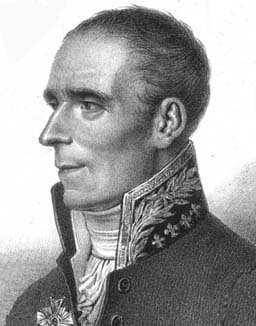
\includegraphics{Laplace.jpg}
\caption{
این مثالی از یک ‎\gls{Action}	 مجاز است.
}
\label{fig:sample1}
\end{figure}

همان‌طور که می‌دانید caption ها اشکال در فهرست اشکال جمع‌آوری می‌شوند، و به احتمال زیاد اولین جایی که واژه Action بکار می‌رود در caption ها است که در فهرست اشکال آورده شده است. پرواضح است که ما نمی‌خواهیم در فهرست اشکال پاورقی داشته باشیم. پس بهتر است که در caption‌ جداول و اشکال از حالت * دستورات استفاده کنیم. یعنی:

\begin{figure}
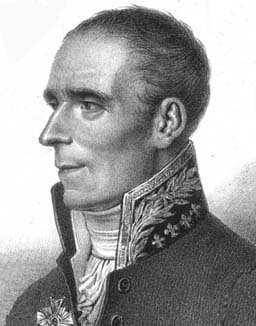
\includegraphics{Laplace.jpg}
\caption{
این مثالی از یک ‪‎\gls*{Action}‬ مجاز است.
}
\label{fig:sample4}
\end{figure}

glsentrytext

این دستور به مانند gls است. با این تفاوت که فقط در متن قسمت text اختصار یا واژه مورد نظر وارد می‌شود، و واژه مورد نظر نه پاورقی می‌خورد و نه در واژه‌نامه‌ها وارد می‌شود. برای واژه و اختصار زیر را در نظر بگیرید.

\newword{Optimization}{Optimization}{بهینه‌سازی}{}
 
\newacronym{DFT}{DFT}{Discrete Fourier Transform}

اکنون اگر در متن خود بنویسید:

می‌توانیم با ‎\glsentrytext{Optimization}‎ تبدیل ‎\glsentrytext{DFT}‎ را

شما در خروجی pdf عبارت زیر را مشاهده خواهید کرد.

می‌توانیم با بهینه‌سازی تبدیل DFT را


اماواژه Optimization و اختصار DFT اگر در این جا حتی اولین باری باشد که بکار رفته باشد، دیگر پاورقی نخواهد خورد، در ضمن این واژه و اختصار وارد واژه‌نامه و فهرست اختصارات نیز نخواهد شد.
glsentryplural

این دستور به مانند glspl است. با این تفاوت که فقط در متن قسمت جمع واژه مورد نظر وارد می‌شود، و واژه مورد نظر نه پاورقی می‌خورد و نه در واژه‌نامه‌ها وارد می‌شود.
glsuseri

اگر از این دستور استفاده کنید، واژه و یا اختصار در متن نمی آید اما در واژه نامه و یا فهرست اختصارات وارد می‌شود. 

\begin{figure}[ht]
\centering
\fbox{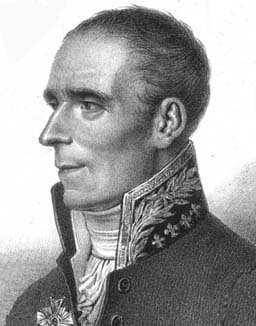
\includegraphics[scale=.5]{Laplace.jpg}}
%\captionsetup{textfont=rm,justification=centering,labelsep=newline}
\caption{\label{fig:laplace} پیر سیمون لاپلاس}
\end{figure}
%\end{document}

  
